\section{Objetivos}

El objetivo de este trabajo se sentrará generar un sistema de sintesis de habla basado en HMMs que sea capaz de sintetizar habla en español con acento extranjero. Una vez obtenidos resultados que consideremos aceptables, procederemos a una etapa de experimentación donde buscaremos \completarObjetivos

\break

\section{Metodología}

En esta sección presentaremos la metodología utilizada para la generación de HMMs, la interpolación entre los mismos y otras tecnicas utilizadas.


A modo de resumen, estos serán los pasos a realizar:


A partir de tres corpus de datos, dos de ellos en castellano y uno en ingles, se realizará un etiquetado fonetico de los corpus para su posterior utilización en el entrenamiento de los HMMs.


Realizar el entrenamiento del sistema. Para esto contaremos con un sistema de sintesis de voz basado en HMM conocido como HTS. 


Una vez generados los HMMs (Uno por cada corpus disponible) utilizaremos herramientas provistas por HTS para interpolar entre ellos y así obtener distintos grados de fonetica y prosodia inglesa a la hora de sintetizar audios.


Dado que el castellano y el ingles no utilizan los mismos simbolos foneticos, si queremos sintetizar audios en castellano con el HMM generado con el corpus en ingles, un desafío que deberemos resolver es el de cubrir todos los simbolos foneticos del castellano por alguno del ingles.

\subsection{Preparación De los datos}


Como ya adelantamos, en este trabajo contamos con tres corpus de datos dispoinbles:


\begin{itemize}
\item secyt-mujer: 741 oraciones, $48$ minutos de habla.
\item loc1\_pal: 1593 oraciones, $2$ horas y $26$ minutos de habla.
\item CMU-ARCTIC-SLT: 1132 oraciones, 56 minutos de habla.
\end{itemize}


Dadas la cantidad de horas de audio disponibles, tanto para loc1\_pal como para CMU-ARCTIC-SLT decidimos utilizar alineamiento forzado para obtener las transcripciones foneticas necesarias para el entrenamiento. Para esto se utilizó Festival y Festvox que a partir de los audios y sus transcripciones grafemicas, permite realizar EHMM alignment sobre el corpus de datos. Para secyt-mujer contabamos previamente con las transcripciones foneticas ya realizadas por lo que decidimos utilizar estas. 


Por otra parte, festival nos permitirá generar features contextuales sobre cada fonema, como el fonema que lo precede, cantidad de palabras en la oración, si la silaba en la que se encuentra esta acentuada, etc. Mas adelante en este trabajo se explicará de que manera son utilizados estos features.


Para este trabajo todos los audios usarán sampling rate de 48kHz, precisión de 16 bits, mono.


% Cosas para hablar:
%TODO: phonetically balanced?
% contextual factors: cuales son, para que sirven.
% desarrollar generacion de uternaces: secty alineaminento mixto: tiempos a mano, features automaticos.
% el etiquetado de cmu\_arctic es en ingles y mapeando al castellano.

\subsection{Entrenamiento Con HTS}

Tanto para el entrenamiento y sintesis del habla se utilizará HTS.


Comenzaremos dando un pequeño resumen del funcionamiento del sistema utilizado:


HTS es un TTS que modela simultaneamente la duración, el espectro (mel-cepstrum) y la frecuencia principal (f0) de manera simultanea utilizando un framework de HMM:

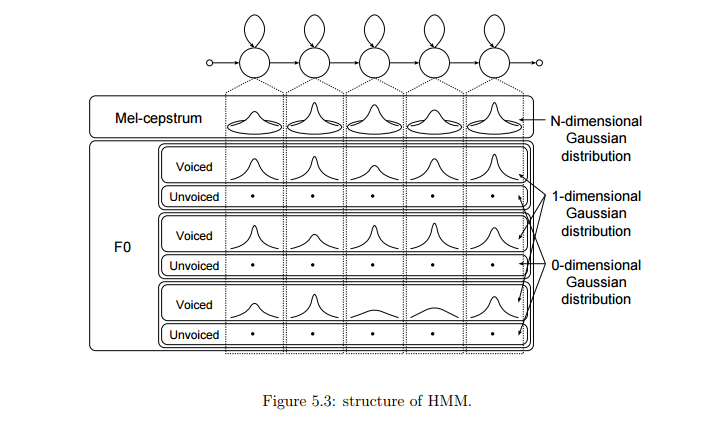
\includegraphics[scale=0.5]{imagenes/hmm.png}


Por otra parte HTS toma la decición de modelar la información prosodica dentro de este mismo framework. Para esto, las distribuciónes para el espectro, la frecuencia principal y las duraciónes son clusterizadas independientemente utilizando tecnicas de aprendisaje automatico y arboles de decición. A continuación se presenta una vista esquematica de la estructura de este nuevo hmm:

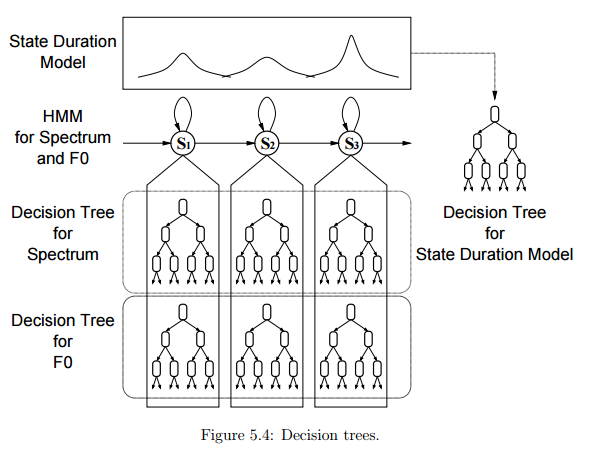
\includegraphics[scale=0.5]{imagenes/hmmContext.png}


En particular para este trabajo el entrenamiento de todos los modelos se realiza utilizando senones (5 fonemas) para los HMM generados.

% Cosas para hablar:
% 5 fonemas.
% hmms
% arboles de decición.
%questions

\subsection{Sintesis utilizando hts\_engine}


Para la sintesis se utilizó hts\_engine, una herramienta de linea de comandos que no solo permite sintetizar oraciones utilizando los modelos acusticos generados sino ademas interpolar entre los distintos HMMs disponibles. Utilizaremos esta herramienta para interpolar entre los HMMs de ingles y castellano para lograr nuevos modelos que mezclen los features acusticos con distintos grados de ingles y de castellano.

Un desafío que se presenta para este trabajo es el mapeo de los fonemas del ingles al castellano. Para empezar, la transcripcion fonetica realizada por festival de las oraciones en ingles puede utilizar 50 simbolos distintos, mientras que la transcripción fonetica del castellano utiliza 31. Habiendo ademas muchos simbolos sin equivalencia. (por ejemplo, con el fonema /rr).

Para resolver esto desarollamos una solución adhoc que consistió en desarrollar una función sobreyectiva que permita tener cubiertos los 31 fonemas del castellano por alguno del ingles.

% Cosas para hablar:
% mapeo utilizado mostrar.
% Expandir en que consiste la interpolación.